\documentclass[11pt,a4paper]{article}

% Self-contained: compiles with pdflatex + the images in figures/.
\usepackage[margin=2.3cm]{geometry}
\usepackage{graphicx}
\usepackage{booktabs}
\usepackage{xcolor}
\usepackage{float}
\usepackage{caption}
\usepackage{tikz}
\usetikzlibrary{arrows.meta,positioning,calc}
\usepackage[hidelinks]{hyperref}

\captionsetup{font=small,labelfont=bf}
\newcommand{\code}[1]{\texttt{#1}}

% Style note (per author request): do not use the double hyphen or the triple
% hyphen anywhere. Ranges are written with the word "to"; asides use commas or
% parentheses. A single hyphen inside a compound word is fine.

\title{\vspace{-1.5em}Real-Time Multi-Camera Digital Twin of Polybags\\
on a Conveyor Belt\\[0.3em]
\large Method, Dataset, and Live Demonstration (Real Track)}
\author{Aw Thura \and Shruti Singh \and Antara Nigudkar\\[0.4em]
\normalsize Autonomous Multisensor Systems, Otto von Guericke University Magdeburg}
\date{September 2026}

\begin{document}
\maketitle

\begin{abstract}
\noindent
This document accompanies the recorded demonstration video of the real track of
the ``Multi-Object Tracking of Polybags'' project. The video shows a live digital
twin of a physical conveyor belt: polybags observed by up to five cameras are
detected, projected onto a shared metric map of the belt, deduplicated across
overlapping cameras, and counted, all in real time and shown on a browser
dashboard. Three recorded scenarios are demonstrated (single moving polybags,
bulk moving polybags, and a timestamped four-camera static capture). This report
describes the detection and calibration method, the datasets used, and, in most
detail, how these parts are integrated into the digital twin. It closes with a
walkthrough of the video and an honest account of what the system does and does
not yet achieve.
\end{abstract}

\section{Purpose and scope}

The real track transfers the perception pipeline from a controllable synthetic
environment to the physical conveyor rig in the Conveyor and Material Technology
Laboratory. The recorded video is the current end-to-end result: it plays back
real camera footage through the full pipeline and visualises, side by side, the
raw per-camera detections and the fused world model of the belt.

Two properties of the real setting shape every design choice, and both are
visible in the video. First, real polybags are a single visual class (there is no
colour that separates one bag from another), so the colour cues that worked in
simulation do not transfer. Second, the cameras are not frame synchronised on the
moving recordings. Both facts push the design away from appearance-based or
timing-based association and towards a geometric solution: calibrate every camera
into one metric belt frame, and reason about bags as positions on the belt.

\section{Method}

The pipeline has four stages: detection, projection onto a calibrated metric belt
map, fusion across cameras, and counting. A live digital twin ties them together.

\subsection{Detection}

Each camera frame is passed through a YOLO object detector (\code{polybag\_v1}, a
YOLO11s detection model). It was trained on the real footage using labels produced
by an automatic labelling pipeline based on a fine-tuned LocateAnything localiser
(the label set \code{labels\_final\_v3}, 7{,}184 boxes over 2{,}926 images,
improved with tiling for dense scenes). On a held-out split the detector reaches a
precision of 0.965, a recall of 0.812, and a mean average precision (mAP50) of
0.864. Those numbers measure agreement with the automatic labels rather than with
human ground truth, since no human-labelled real test set exists, and they should
be read that way. The detector runs at an image size of 512 with a confidence
threshold of 0.25.

\subsection{Calibration and the metric belt map}

The shared coordinate frame is a top-down metric map of the conveyor, built from a
tape-measure survey of the belt rather than from any single camera. Its origin is
the centre of a calibration board placed under the \code{basler\_1} camera, with
the $+Y$ axis running along the belt in the travel direction and the $+X$ axis
running across it. Intrinsics are solved per camera from ChArUco board captures;
extrinsics are solved board-free by registering one still frame per camera to the
surveyed map. Every detection is turned into a belt position by undistorting its
reference pixel (the bounding-box centre) and applying the camera's plane
homography to the belt.

Calibration quality differs by camera, and the video reflects this. The two Basler
cameras are solved as metric (full pose). The Lucid and the RealSense colour
cameras are homography-only: they have a plane mapping to the belt but not a full
metric pose, so their across-belt position is less reliable. The dashboard marks
these cameras as ``homography'' and treats them accordingly.

\subsection{Fusion across cameras}

Where two cameras see the same bag (the two Basler cameras overlap near the belt
entry), their detections must be merged into one object. The fusion stage does
this by cross-camera deduplication: detections closer than a fixed gate are merged
into a single object, but only if they come from different cameras. Two detections
from the same camera are never merged, because the per-camera tracker has already
established that they are distinct bags. The merged objects are then given
persistent identities by greedy nearest-neighbour tracking on the belt plane.

Carrying a single identity for a bag across the blind gap between the upstream
Basler view and the downstream Lucid view is a genuine re-identification problem,
which is out of scope for this demonstration and is switched off. The dashboard
states this explicitly (``re-ID off''). The counting method below is chosen so
that it does not depend on solving it.

\subsection{Counting}

The belt carries many bags at once (up to twelve to twenty one per frame in the
bulk scenario), and it moves quickly (about 440 mm per second). At the pipeline's
inference rate a bag travels roughly as far between frames as the spacing between
neighbouring bags, so counting each bag by tracking it across a single line is
unreliable. The system therefore counts by flux: it integrates how much detection
occupancy accumulates in a thin band around a counting line over time, and divides
by how long a single bag lingers in that band (the band thickness divided by the
belt speed). This is an occupancy-flow estimate that needs no per-bag identity and
tolerates dense, fast flow. The belt speed is measured live from the motion of the
detections, not tuned. Two counting lines are used, one near the belt entry and
one near the exit, and the displayed count is written with a preceding ``$\approx$''
to signal that it is an estimate. A simple per-track line-crossing count is kept
beside it, in small grey text, as a reference; it under-counts badly, which is
exactly why flux is the primary method.

\section{Dataset details}

The footage was recorded on the physical rig and provided by the project
supervisor. The rig carries five cameras, all recording at a resolution of
1280 by 720, over a belt that is 580 mm wide. Table~\ref{tab:cameras} lists the
cameras and their calibration status. Three recorded scenarios are shown in the
video; Table~\ref{tab:scenarios} summarises them.

\begin{table}[H]\centering
\caption{The five cameras of the rig and their calibration status.}
\label{tab:cameras}
\begin{tabular}{lll}
\toprule
Camera & Type & Calibration \\
\midrule
\code{basler\_1}     & Basler GigE (near top-down)   & metric (full pose) \\
\code{basler\_2}     & Basler GigE (oblique)         & metric (full pose) \\
\code{lucid}         & Lucid Triton GigE (downstream)& homography-only \\
\code{rgbd\_1\_color}& Intel RealSense D435 colour   & homography-only \\
\code{rgbd\_2\_color}& Intel RealSense D435 colour   & not used here \\
\bottomrule
\end{tabular}
\end{table}

\begin{table}[H]\centering
\caption{The three demonstrated scenarios. The moving recordings predate the
timestamp recorder and so are played on an approximate shared timeline; the static
recording carries per-frame device timestamps and is played in true synchrony.}
\label{tab:scenarios}
\begin{tabular}{llll}
\toprule
Scenario & Session & Cameras & Notes \\
\midrule
single & \code{20260528\_092854} & basler\_1, basler\_2, lucid & moving, one bag flow, no timestamps \\
bulk   & \code{20260528\_100631} & basler\_1, basler\_2, lucid & moving, dense pile, no timestamps \\
static & \code{20260731\_124825} & four colour cameras         & static bags, true timestamp sync \\
\bottomrule
\end{tabular}
\end{table}

There is one gap worth stating plainly: no recording is both moving and
timestamped. The moving scenarios have the interesting motion but only an
approximate synchronisation, while the timestamped scenario has true
synchronisation but nearly static bags. A future capture that is both moving and
timestamped would remove this limitation.

\section{Integration with the digital twin}

The digital twin is where detection, calibration, fusion, and counting come
together as one live system. It is built as two decoupled programs joined by a
lightweight message bus, sketched in Figure~\ref{fig:pipeline}.

\begin{figure}[H]\centering
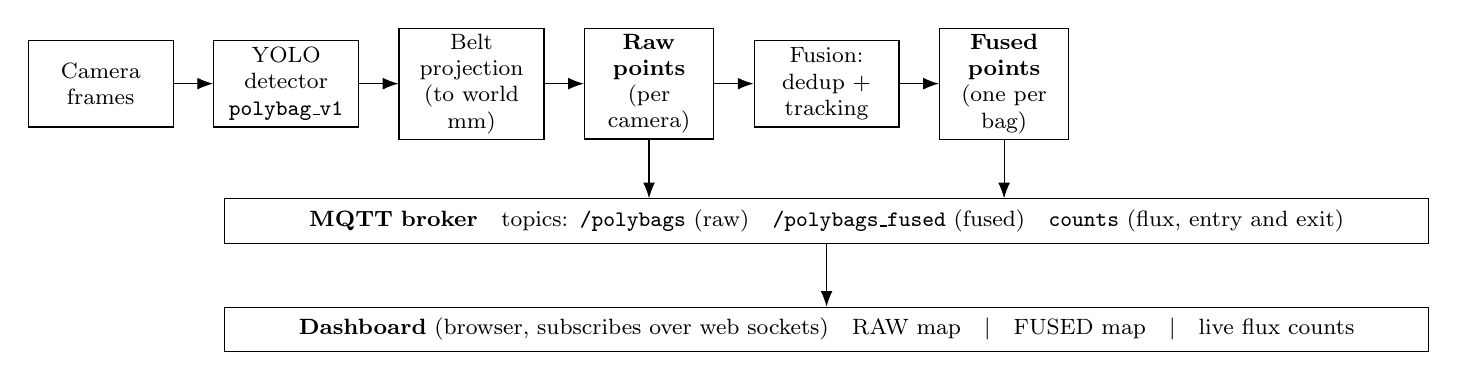
\begin{tikzpicture}[font=\footnotesize,>={Latex[length=2mm]},
  proc/.style={draw,fill=white,align=center,
    minimum height=11mm,text width=17mm,inner sep=2pt},
  model/.style={proc},
  pts/.style={draw,fill=white,align=center,
    minimum height=11mm,text width=15mm,inner sep=2pt},
  bus/.style={draw,fill=white,align=center,inner sep=4pt},
  cons/.style={draw,fill=white,align=center,inner sep=4pt}]
% top row: the producer pipeline
\node[proc] (cam) {Camera\\frames};
\node[model,right=5mm of cam] (det) {YOLO\\detector\\\texttt{polybag\_v1}};
\node[proc,right=5mm of det] (proj) {Belt\\projection\\(to world mm)};
\node[pts,right=5mm of proj] (raw) {\textbf{Raw}\\\textbf{points}\\(per camera)};
\node[proc,right=5mm of raw] (fus) {Fusion:\\dedup +\\tracking};
\node[pts,right=5mm of fus] (fused) {\textbf{Fused}\\\textbf{points}\\(one per bag)};
\draw[->] (cam)--(det); \draw[->] (det)--(proj); \draw[->] (proj)--(raw);
\draw[->] (raw)--(fus); \draw[->] (fus)--(fused);
% MQTT bus, fed by raw and fused
\node[bus,below=9mm of fus,text width=150mm] (mqtt) {\textbf{MQTT broker}\quad
  topics: \texttt{/polybags} (raw)\quad \texttt{/polybags\_fused} (fused)\quad
  \texttt{counts} (flux, entry and exit)};
\draw[->] (raw.south) -- (raw.south|-mqtt.north);
\draw[->] (fused.south) -- (fused.south|-mqtt.north);
% consumer
\node[cons,below=8mm of mqtt,text width=150mm] (dash) {\textbf{Dashboard}
  (browser, subscribes over web sockets)\quad
  RAW map $\;|\;$ FUSED map $\;|\;$ live flux counts};
\draw[->] (mqtt)--(dash);
\end{tikzpicture}
\caption{The digital-twin pipeline. Each camera frame is run through the YOLO
detector (the model), and every detection is projected onto the metric belt map,
giving the per-camera \emph{raw points}. Fusion deduplicates these across cameras
and tracks them into \emph{fused points} (one per bag). The producer publishes
raw points, fused points, and the flux counts over MQTT, and the browser dashboard
subscribes and draws the RAW and FUSED maps side by side.}
\label{fig:pipeline}
\end{figure}

\paragraph{Producer (streamer).}
A background service plays the selected scenario's camera videos in synchrony,
runs the detector on each frame, projects every detection onto the metric belt map
through that camera's calibration, assigns per-camera identities, runs the fusion
and counting stages, and publishes the results. It also serves each camera's
annotated video as a live image stream, with the detection overlay drawn on the
same frame it was inferred from so that the boxes never lag the bags. On the
development machine it sustains roughly five inference updates per second across
three cameras at an image size of 512.

\paragraph{Transport.}
Results are published over MQTT. The producer publishes the raw per-camera
positions on one topic and the fused world objects on another, together with the
running counts and the playback state, on a steady schedule that is decoupled from
the irregular inference rate. This keeps the dashboard smooth even when inference
is slow.

\paragraph{Consumer (dashboard).}
A browser page subscribes to both topics over web sockets and draws everything on
the clean metric belt map. It is fully decoupled from the producer, so any source
that speaks the same messages would drive it. The layout, seen in every figure,
places the live camera feeds on the left and two synchronised maps on the right:
a RAW map that shows one dot per camera detection, coloured by camera, and a FUSED
map that shows one object per bag after deduplication. The two green dashed lines
are the entry and exit counting lines, and each carries its live flux count. A
legend states which cameras are metric and which are homography-only, and confirms
that re-identification is off. Playback controls (Play, Pause, and a Loop toggle)
let the operator freeze the twin or let it loop; pausing freezes the feeds, the
map, and the counts together.

The end-to-end path for a single bag is therefore: a pixel in one camera, to an
undistorted pixel, to a millimetre position on the belt through the calibration,
to a fused world object after deduplication, to a contribution to the flux count,
to a dot on the live map. The same calibration code that placed the cameras drives
the projection at run time, so there is a single source of truth for the geometry.

\section{Walkthrough of the recorded video}

The video runs the three scenarios in turn, restarting the producer between them
to switch datasets, and shows the dashboard throughout.

\subsection{Single moving polybags}

Figure~\ref{fig:single} is a frame from the single scenario. All three cameras
detect bags: the \code{basler\_1} boxes are red, \code{basler\_2} green, and
\code{lucid} blue, matching their dots on the RAW map. At this instant the RAW map
holds fifty detections while the FUSED map holds twenty four objects: the drop is
the cross-camera deduplication merging the overlapping Basler views into one object
per bag. The entry and exit flux counts read about twenty five and about eighteen,
with the much smaller per-track crossing counts shown in grey beside them.

\begin{figure}[H]\centering
\includegraphics[width=\textwidth]{figures/single_overview.png}
\caption{Single moving polybags. Left: the three live camera feeds with
per-camera detection boxes. Right: the RAW map (one dot per detection, coloured by
camera) beside the FUSED map (one object per bag after cross-camera
deduplication). The green dashed lines are the entry and exit counting lines with
their live flux counts.}
\label{fig:single}
\end{figure}

\subsection{Bulk moving polybags}

Figure~\ref{fig:bulk} is a frame from the bulk scenario, where a dense pile of
bags crosses the belt. Both Basler feeds are packed with overlapping bags, and the
RAW map is correspondingly crowded. This is the case that defeats per-track
crossing counts and motivates the flux method: with this many bags moving this
quickly, no per-bag tracker can keep them separate at the available frame rate, but
the occupancy-flux estimate still recovers a count in the right range.

\begin{figure}[H]\centering
\includegraphics[width=\textwidth]{figures/bulk_dense.png}
\caption{Bulk moving polybags. A dense pile fills the two Basler views. The scene
carries far more bags at once than a per-track counter can individuate at the
inference rate, which is why the throughput count is estimated by occupancy flux
rather than by counting line crossings.}
\label{fig:bulk}
\end{figure}

\subsection{Static, four-camera, timestamped}

Figure~\ref{fig:static} is a frame from the static scenario. Here all four colour
cameras are active, including \code{rgbd\_1\_color}, and the recording carries
per-frame device timestamps, so the cameras are played in true synchrony (marked
``true sync'' in the header). The bags are nearly static, so this scenario is less
about motion and more about showing the full four-camera projection and fusion
onto the shared belt map at once.

\begin{figure}[H]\centering
\includegraphics[width=\textwidth]{figures/static_4cam.png}
\caption{Static, timestamped, four-camera capture. All four colour cameras project
onto the shared belt map in true synchrony. This scenario exercises the full
multi-camera geometry, including the homography-only Lucid and RealSense cameras.}
\label{fig:static}
\end{figure}

\section{What the demonstration shows, and its limits}

The video demonstrates a working real-time pipeline: real footage from up to four
cameras is detected, projected into one metric belt frame, deduplicated across
overlapping views into a single world model, counted by occupancy flux, and shown
live with interactive playback. The RAW versus FUSED comparison makes the
cross-camera deduplication visible, and the counting lines show a throughput
estimate that survives dense, fast flow.

The honest limitations are these. The detector's recall is imperfect and depends
on the camera, so the counts are estimates rather than exact figures. Two of the
cameras are homography-only, so their across-belt positions are less accurate than
the metric Basler cameras. Identity is not carried across the blind gap between the
upstream and downstream camera sets, which is a deferred re-identification problem.
The moving recordings are only approximately synchronised. And the whole pipeline
runs on a single laptop, which caps the inference rate and, through it, the
achievable counting accuracy. The clearest path to a more accurate count is better
detector recall rather than a more elaborate tracker.

\section{Reproducing the demonstration}

The system lives in \code{real\_polybags/algorithm/}. A local MQTT broker is
started first (\code{mosquitto}), then the producer is launched with a chosen
scenario, for example \code{--scenario single}, \code{--scenario bulk}, or
\code{--scenario static}, and the dashboard is opened in a browser at the local
address the producer prints. The detector model, the counting lines, the counting
band, and the fusion settings are all set in one configuration file, so the
behaviour shown in the video can be reproduced or adjusted without changing code.

\end{document}
